% Frank.Nielsen@acm.org
 
\documentclass[11pt]{article}
\usepackage{fullpage,amssymb,amsmath,hyperref,url,graphicx}

\def\eqdef{:=}
\def\eqnota{:=:}
\def\dnu{\mathrm{d}\nu}
\def\calX{\mathcal{X}}
\def\bbR{\mathbb{R}}
\def\Var{\mathrm{Var}}
\def\leftsup#1{{}^{#1}}\def\calH{\mathcal{H}}
\def\calS{\mathcal{S}}
\def\calP{\mathcal{P}}
\def\calF{\mathcal{F}}
\def\calY{\mathcal{Y}}
\def\calS{\mathcal{S}}

\def\diag{\mathrm{diag}}

\def\bbX{\mathbb{X}}

\def\codeDist#1{\fbox{#1}}

\def\Mult{\mathrm{Mult}}
\def\rightarrowDist{\stackrel{d}{\longrightarrow}}

\def\dnu{\mathrm{d}\nu}

\def\st{{\ :\ }}
\def\suchthat{\mbox{\ such that\ }}

\def\inner#1#2{\langle #1,#2\rangle}
\def\innerThree#1#2#3{\inner{#1}{#2}_{#3}}

\def\bbR{\mathbb{R}}

\def\dz{\mathrm{d}z}
\def\dx{\mathrm{d}x}
\def\dy{\mathrm{d}y}
\def\ds{\mathrm{d}s}
\def\dt{\mathrm{d}t}
\def\dtheta{\mathrm{d}\theta}
\def\deta{\mathrm{d}\eta}

\def\connectionTypeOrder#1#2{{\stackrel{#1}{\nabla}^{#2}}}

\def\matrixthreethree#1#2#3#4#5#6#7#8#9{\left[\begin{array}{lll}#1 & #2 & #3\cr #4 & #5 & #6\cr #7 & #8 & #9\end{array}\right]}
\def\mattwotwo#1#2#3#4{\left[\begin{array}{ll}#1&#2\cr #3 & #4\end{array}\right]}


\newenvironment{proof}{\paragraph{Proof:}}{\hfill$\square$}

 \newtheorem{Remark}{Remark}
\newtheorem{Proposition}{Proposition}

\sloppy


\title{The symmetrized Bregman divergence\\ as dual geodesic energy functionals\thanks{Extracted from ongoing working notes~\cite{IG4ML}.}}

\date{June 2022}

\author{Frank Nielsen\\ {\tt Frank.Nielsen@acm.org}}

\begin{document}
\maketitle

The Bregman divergence~\cite{Bregman-1967} between two vector parameters $\theta_1$ and $\theta_2$ induced by strictly convex function $F(\theta)$ is $B_F(\theta_1:\theta_2):=F(\theta_1)-F(\theta_2)-(\theta_1-\theta_2)^\top \nabla F(\theta_2)$.
Let $\eta=\nabla F(\theta)$ and $\theta=\nabla F^*(\eta)$ denote the dual parameterizations obtained by the Legendre-Fenchel convex conjugate  $F^*(\eta)$ of $F(\theta)$.
The Jeffreys-type symmetrization\footnote{To distinguish it with the Jensen-Shannon type symmetrization~\cite{JSD-2019}.} (i.e., arithmetic symmetrization of the sided Bregman divergences~\cite{SBD-2009}) of the Bregman divergence is defined by
$$
S_F(\theta_1;\theta_2):=B_F(\theta_1:\theta_2)+B_F(\theta_2:\theta_1)=(\theta_2-\theta_1)^\top (\eta_2-\eta_1)=S_{F^*}(\eta_1;\eta_2),
$$
 
 \begin{figure}[hb]%
\centering
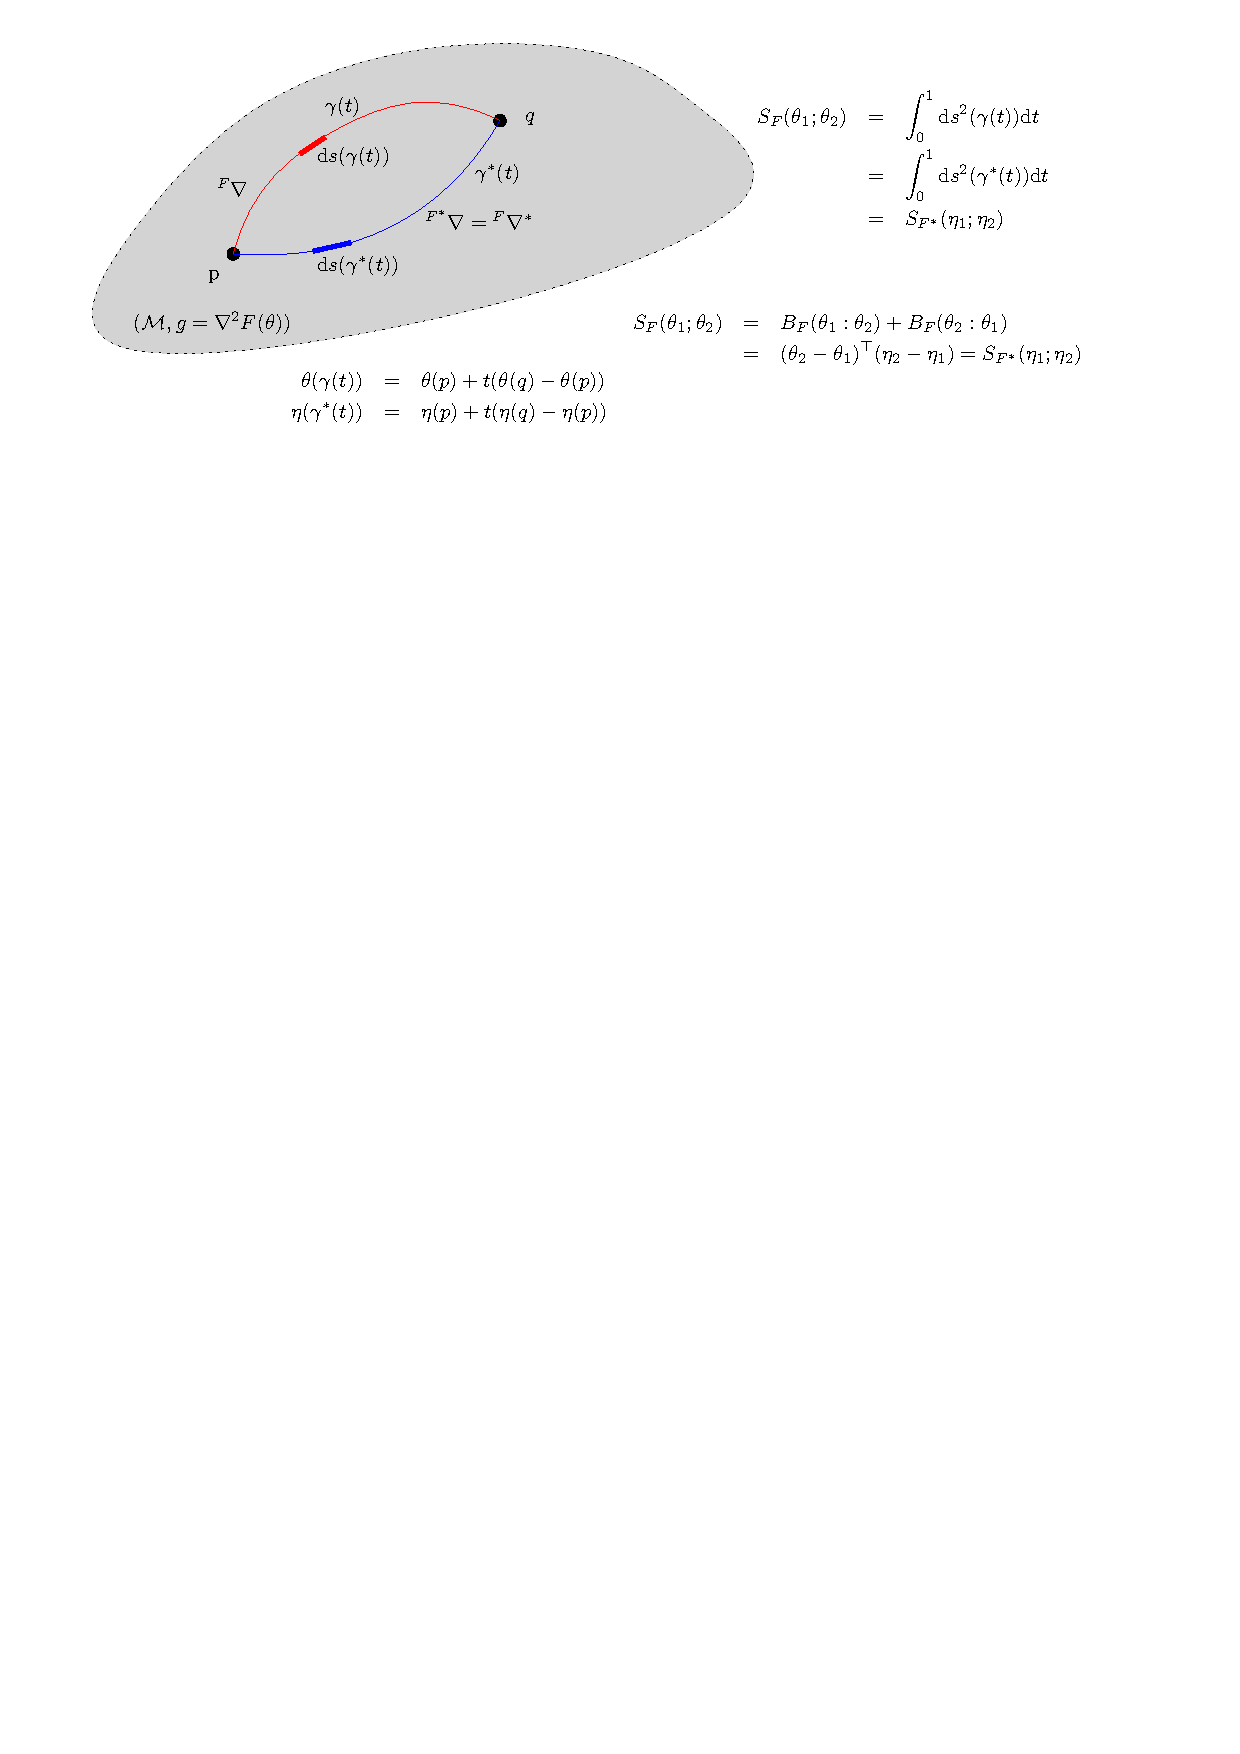
\includegraphics[width=0.75\columnwidth]{FigIpe-SBDGeodesicsEnergy.pdf}%
\caption{The symmetrized Bregman divergence $S_F(\theta_p;\theta_q)$ can be interpreted as the energy of the Hessian metric along the primal or dual geodesics linking $p$ to $q$.}%
\label{fig:DualGeodesicEnergy}%
\end{figure}


 

\begin{Proposition}[Theorem 3.2 of~\cite{IG-2016}, illustration in Figure~\ref{fig:DualGeodesicEnergy}]
The Jeffreys-Bregman divergence $S_F(\theta_1;\theta_2)$ is interpreted as the energy induced by the Hessian metric $\nabla^2 F(\theta)$ on the dual geodesics:
$$
S_F(\theta_1;\theta_2)=\int_0^1 \ds^2(\gamma(t))\dt=\int_0^1 \ds^2(\gamma^*(t))\dt.
$$ 
\end{Proposition}


\begin{proof}
The proof is based on the first-order and second-order directional derivatives.
The first-order directional derivative $\nabla_u F(\theta)$ with respect to vector $u$ is defined by 
$$
\nabla_u F(\theta)=\lim_{t\rightarrow 0} \frac{F(\theta+tv)-F(\theta)}{t}=v^\top \nabla F(\theta).
$$
 
The second-order directional derivatives $\nabla_{u,v}^2 F(\theta)$ is
\begin{eqnarray*}
\nabla_{u,v}^2 F(\theta) &=& \nabla_{u} \nabla_v F(\theta),\\
 &=& \lim_{t\rightarrow 0} \frac{v^\top \nabla F(\theta+tu)-v^\top\nabla F(\theta)}{t},\\
&=& u^\top \nabla^2 F(\theta) v.
\end{eqnarray*}


Now consider the squared length element $\ds^2(\gamma(t))$ on the primal geodesic $\gamma(t)$ expressed using the primal coordinate system $\theta$:
$\ds^2(\gamma(t))=\dtheta(t)^\top \nabla^2F(\theta(t)) \dtheta(t)$ with $\theta(\gamma(t))=\theta_1+t(\theta_2-\theta_1)$ and $\dtheta(t)=\theta_2-\theta_1$.
Let us express the $\ds^2(\gamma(t))$   using the second-order directional derivative:
$$
\ds^2(\gamma(t))=\nabla^2_{\theta_2-\theta_1}  F(\theta(t)).
$$
Thus we have $\int_0^1 \ds^2(\gamma(t))\dt=[\nabla_{\theta_2-\theta_1}  F(\theta(t))]_0^1$,
where the first-order directional derivative is $\nabla_{\theta_2-\theta_1}  F(\theta(t))=(\theta_2-\theta_1)^\top \nabla F(\theta(t))$.
Therefore we get $\int_0^1 \ds^2(\gamma(t))\dt=(\theta_2-\theta_1)^\top (\nabla F(\theta_2)-\nabla F(\theta_1))=S_F(\theta_1;\theta_2)$.

Similarly, we express the squared length element $\ds^2(\gamma^*(t))$ using the dual coordinate system $\eta$ as the second-order directional derivative of $F^*(\eta(t))$ with $\eta(\gamma^*(t))=\eta_1+t(\eta_2-\eta_1)$:
$$
\ds^2(\gamma^*(t))=\nabla^2_{\eta_2-\eta_1}  F^*(\eta(t)).
$$
Therefore, we have  $\int_0^1 \ds^2(\gamma^*(t))\dt=[\nabla_{\eta_2-\eta_1}  F^*(\eta(t))]_0^1=S_{F^*}(\eta_1;\eta2)$.
Since $S_{F^*}(\eta_1;\eta_2)=S_F(\theta_1;\theta_2)$, we conclude that
$$
S_F(\theta_1;\theta_2)=\int_0^1 \ds^2(\gamma(t))\dt=\int_0^1 \ds^2(\gamma^*(t))\dt
$$

In 1D, both pregeodesics $\gamma(t)$ and $\gamma^*(t)$ coincide. We have $\ds^2(t)=(\theta_2-\theta_1)^2 f''(\theta(t))=(\eta_2-\eta_1){f^*}''(\eta(t))$ so that we check that $S_F(\theta_1;\theta_2)=\int_0^1 \ds^2(\gamma(t))\dt=(\theta_2-\theta_1)[f'(\theta(t))]_0^1=(\eta_2-\eta_1)[{f^*}'(\eta(t))]_0^1=(\eta_2-\eta_1)(\theta_2-\theta_2)$.
\end{proof}


\begin{Remark}
In Riemannian geometry, a curve $\gamma$ minimizes the energy $E(\gamma)=\int_0^1 |\dot\gamma(t)|^2\dt$ if it minimizes the length $L(\gamma)=\int_0^1 \|\dot\gamma(t)\|\dt$ and $\|\dot\gamma(t)\|$ is constant. Using Cauchy-Schwartz inequality, we can show that $L(\gamma)\leq E(\gamma)$.
\end{Remark}

\bibliographystyle{plain}
\bibliography{SBDdualGeodesicFunctionalBIB}
\end{document}
